\chapter{Method and materials}


\section{Study species} %Usikker på om eg skal ha med
%\subsubsection{Rev}  ?

%We also collated information on average body and home range sizes for a subset of species surveyed in the reviewed studies in order to better quantify the functional diversity of wildlife being sampled by CTs and to evaluate the degree to which CT methodologies were tailored to focal species. Burton 2015

The species I'll focus on in this thesis are the species that most frequently was observed \emph{(>50 events)}, excluding farmed animals (e.g. cattle), humans and dogs, and grouped categories of animals (e.g. birds).
Given that the decisions on camera placement (height and angle) were made with the aim on photo capturing lynx(), I have also excluded smaller species from the analysis.
% Idea sprung from reading Meek 2014 guiding principles; Height of camera and, distance to centre of detection zone or lure. Growing skeptical to the validity of my argument now that I know about the random effect in models. As I argued in my own notes when reading the Meek article I don't think I need to "take these biases into consideration" because I'm trying to detect differences between the same cameras.
This includes three species, squirrel(), hare() and European pine marten\textit{(Martes martes)}. 
Though they showed up frequently on many locations, there are inevitably some cameras that are too biased towards larger animals, resulting in an inconsistency of their detection rates. 
In turn, it is difficult to distinguish whether the species was affected by the white LED or not, as they could have triggered the camera, but already escaped the frame. %TODO må tygge litt på det argumentet.

In the end, the species I have used in my analyses are roe deer\textit{()}, red fox\textit{()}, badger\textit{(Meles meles)}, moose\textit{()}, red deer\textit{(Cervus elaphus)} and lynx. 

\section{Study area} %TODO 
%mogleg å kjøre ein fin overgang fra intro til study area? Study area valt pga dårlige snøforhold -> vanskelig å gjere spor-tellinger (\cite{Odden2015})


%https://klimaservicesenter.no/faces/desktop/article.xhtml?uri=klimaservicesenteret/klimaprofiler/klimaprofil-oslo-og-akershus
%https://klimaservicesenter.no/faces/desktop/article.xhtml?uri=klimaservicesenteret%2Fklimaprofiler%2Fklimaprofil-buskerud  
The study area (59.36-60.47° N, 9.43-10.91° E) %berre eit grovt overslag
extends over much of the southeastern parts of Norway in counties Flå, Krødsherad, Sigdal, Ringerike, Modum, Hole, Lier, Øvre Eiker, Asker, Oslo, Enebakk, Indre Østfold, Våler, Råde, Moss, Frogn and Vestby.
The climate has a continental character due to rain shadows of the mountain ridges from the west. 

The mean annual temperatures ranges from 2-6\celsius  and precipitation lies between 700-1500mm (\cite{Moen1999}). 
Topography is predominantly flat towards the south, and more rugged and elevated towards the north. The landscape is a mosaic of forest and agricultural areas, divided with a wide network of gravel roads.
The area is situated in the southern boreal and the boreonemoral zones. %Må finne oppdaterte data (frå Norges vassdrags- og energidirektorat, 2019?)

Norway spruce (\textit{Picea abies}) and Scots pine (\textit{Pinus sylvestris}) make up the dominating boreal coniferous forests, with frequent presence of silver birch (\textit{Betula pendula}) and downy birch (\textit{Betula pubescens}), then aspen (\textit{Populous tremula}), alder (\textit{Alnus incana}) and black alder (\textit{Alnus glutinosa}).

Growing season length 170 - 190 days (Moen, 1999, map 6, s.21) %må finne oppdaterte data
Snow cover length												%må finne oppdaterte data %TODO

Most cameras were set in forest areas, usually by a tractor path or human trail, sometimes by animal paths. Their distance from houses or roads varied to a large extent, and some areas were logged (ved Vansjø) and even greatly changed under development of new infrastructure (toglinje på nordligste kamera ~1255)


\section{Study design} %TODO
For the study I chose 60 already established camera sites with infrared light(Reconyx and Browning models). The cameras had been installed on trees 1-3 meters from human or tractor paths, 40-120 cm above ground level, with the original aim to photo capture lynx (\cite{Odden2015}). 
I divided the sites randomly into three groups of 20 cameras. Cameras in group A remained unchanged, whilst group B and C were equipped with an additional white LED camera (Reconyx PC850) in alternating 3 month-periods, as shown in figure\vref{fig:exp_set}.

\begin{figure}
    \begin{center}
    	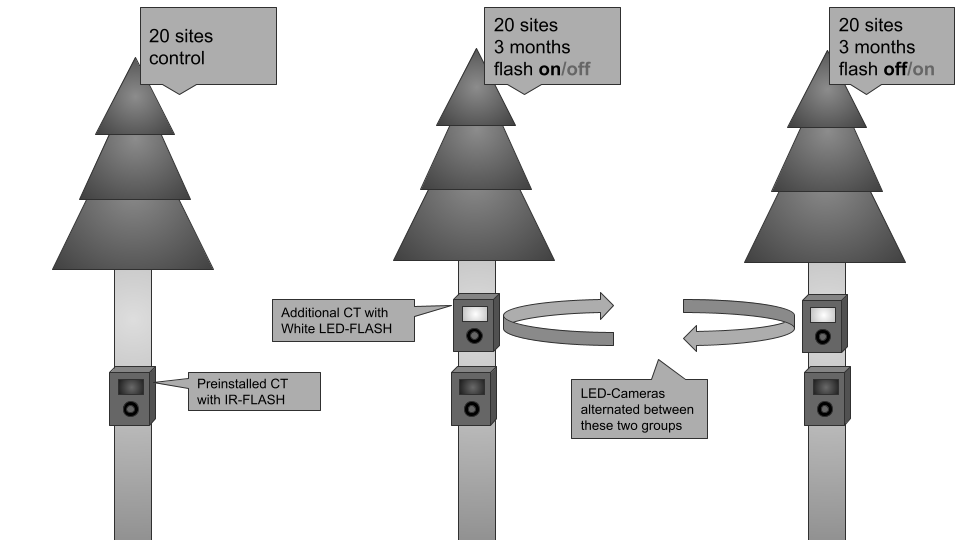
\includegraphics[scale=0.3]{./img/experiment_setup.png} %insert figure of groups     
    \end{center}
    	\caption[Experiment setup]%
    	{Experiment setup \par \small I chose 60 sites with preinstalled IR Camera Traps (CTs) for my study, and divided them into three groups, where the first group remained unchanged as a control, and the two other alternated on having an additional white LED camera present. In the end, seven CTs were removed from the analysis due to large gaps in the data, etc.}
    \label{fig:exp_set}
\end{figure}

%TODO Insert timeserie-plot of all cameras with period 1_1 0_1 and so on.

The preinstalled cameras were set up and handled by people from the Norwegian Institute of Nature Research (NINA) and --- at the sites further from Oslo  --- by members of the Norwegian Hunters and Fishers Society (NJFF). 
%as a conflict mitigating strategy. %%Kan kuttes. Evt må det forklares
The installation of the cameras did not follow a strict protocol, nor were their locations chosen randomly. The overall placement was systematic as decided by NINA, then there was a deliberately-biased placement of the CTs put up in areas where the individual handler deemed it most likely to photograph lynx, and hence, based on a combination of site accessibility and expectations of animal occurence %(\cite{Burton2015} ). %TODO vask språket

%\emph{presence of natural or artificial attractants may draw animals in to a CT} \cite{Burton2015}.

As shown in figure\vref{fig:exp_set}, I set up all white LED cameras above the cameras already in place. 
However, at the particular site shown in figure\vref{fig:cam_ex_c} the infrared camera had been installed so far above ground level that I chose to position the white LED camera below the camera already in place. %endra på av Atle, men kan vaskas ytterligere 
For the periods without white flash treatment, I moved the cameras to their next site. However, the boxes installed on the trees remained (see figure \ref{fig:cam_ex_d}).
First, I equipped Group B with an additional white LED as seen in \vref{fig:cam_ex_main}. After approximately three months, I moved the white LED cameras to group C. These two periods were both marked as period 1-1, as seen in \vref{fig:period_timeseries}. %TODO insert facet-plot of flash-periods, and one plot of all control-cameras coloured in their control_period.
The camera boxes remained at each site untill the end of the experiment. Note that group C had no extra boxes before the start of their first period in May 2019 (i.e. remained identical to the control group A untill May). 

\begin{figure}
	\label{fig:period_timeseries}
\end{figure}

I visited sites of group B and C at least once every three months in order to move the LED cameras. For logistical reasons I visited sites of group A less often. %Her trengs ein språkleg endring
However, as the cameras were part of other, ongoing projects, they were occasionally visited by other workers from NINA to retreive the Secure Digital memory cards (hereby SD Cards) for data. %write in full on first mention (-Atle)
This was mostly the case for sites close to, and south of, Oslo, or rather, the cameras not normally operated by members of the NJFF.

When doing the analyses I needed periods of similar lengths to each other. Therefore, I divided the control group-cameras into four periods of similar lengths to that of the cameras with white LED periods (see figure \vref{fig:period_timeseries}).





\begin{figure}
		\begin{subfigure}{.5\textwidth}
		  \centering
		  	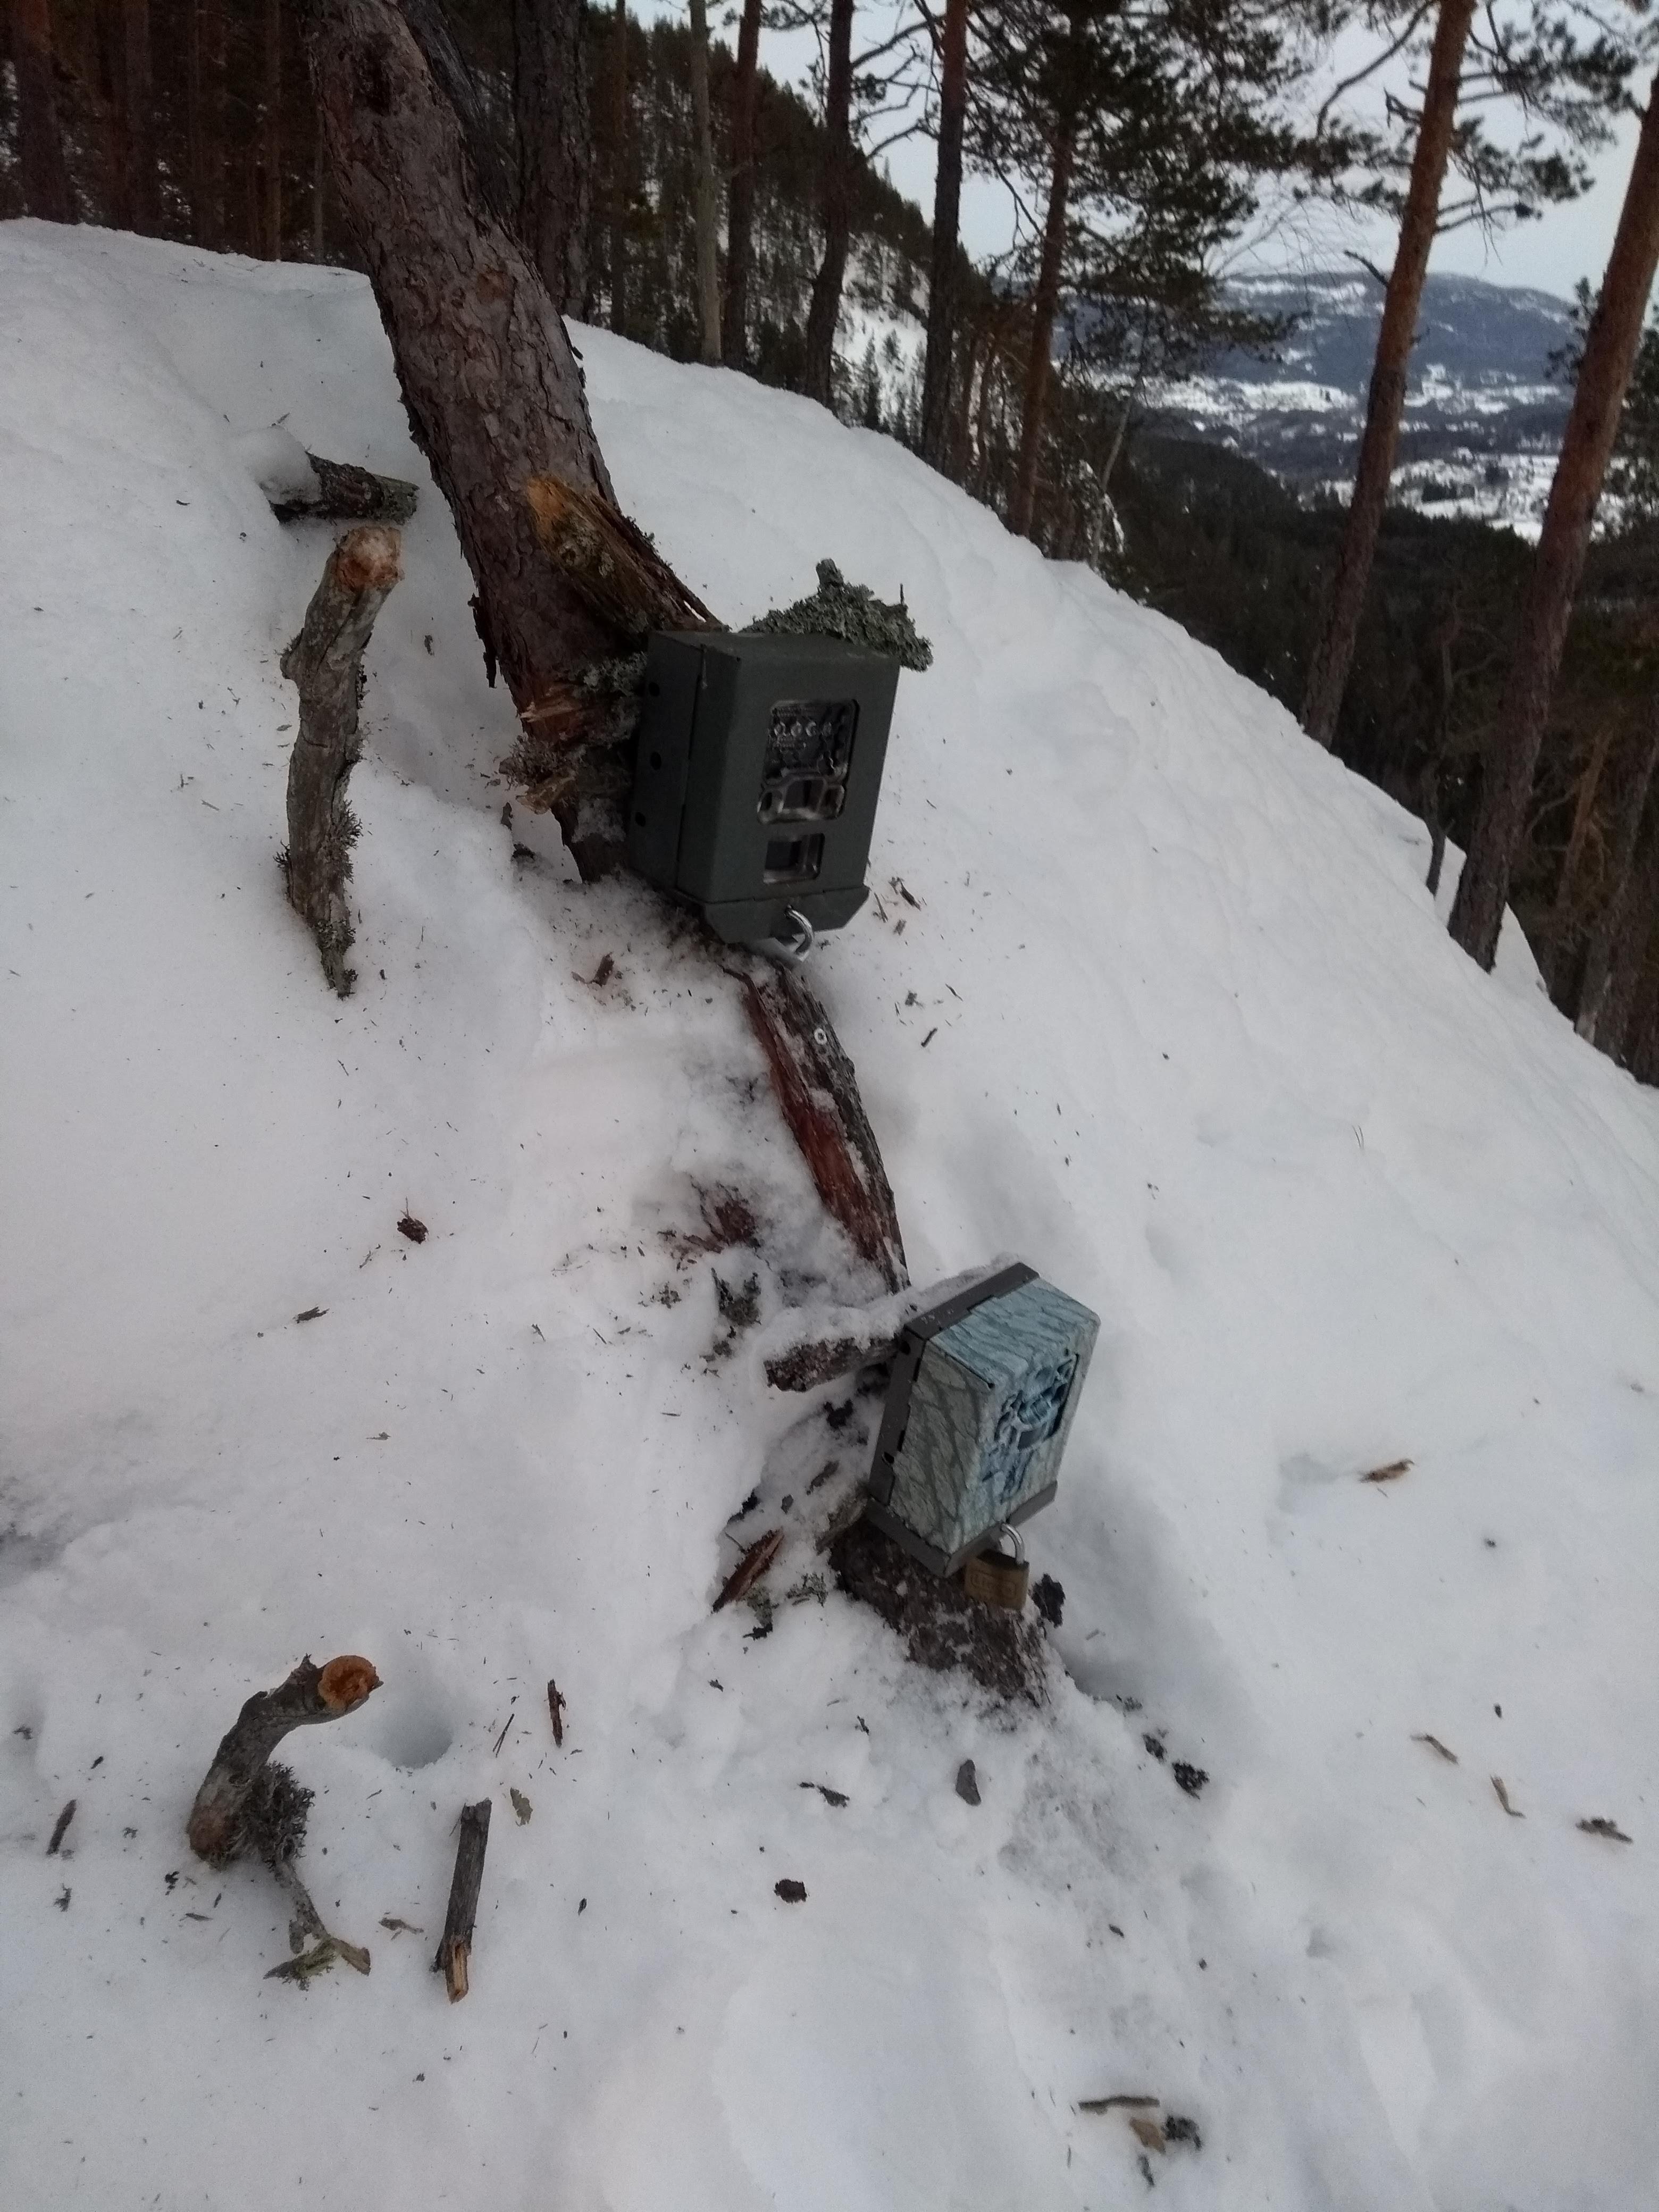
\includegraphics[width=.8\linewidth]{./img/cam_install_example/IMG_20190212_161615169.jpg}
		  \caption{Browning infrared,\\ installed on a fallen tree}
		  	\label{fig:cam_ex_a}
	\end{subfigure}
		\begin{subfigure}{.5\textwidth}
		  \centering
		  	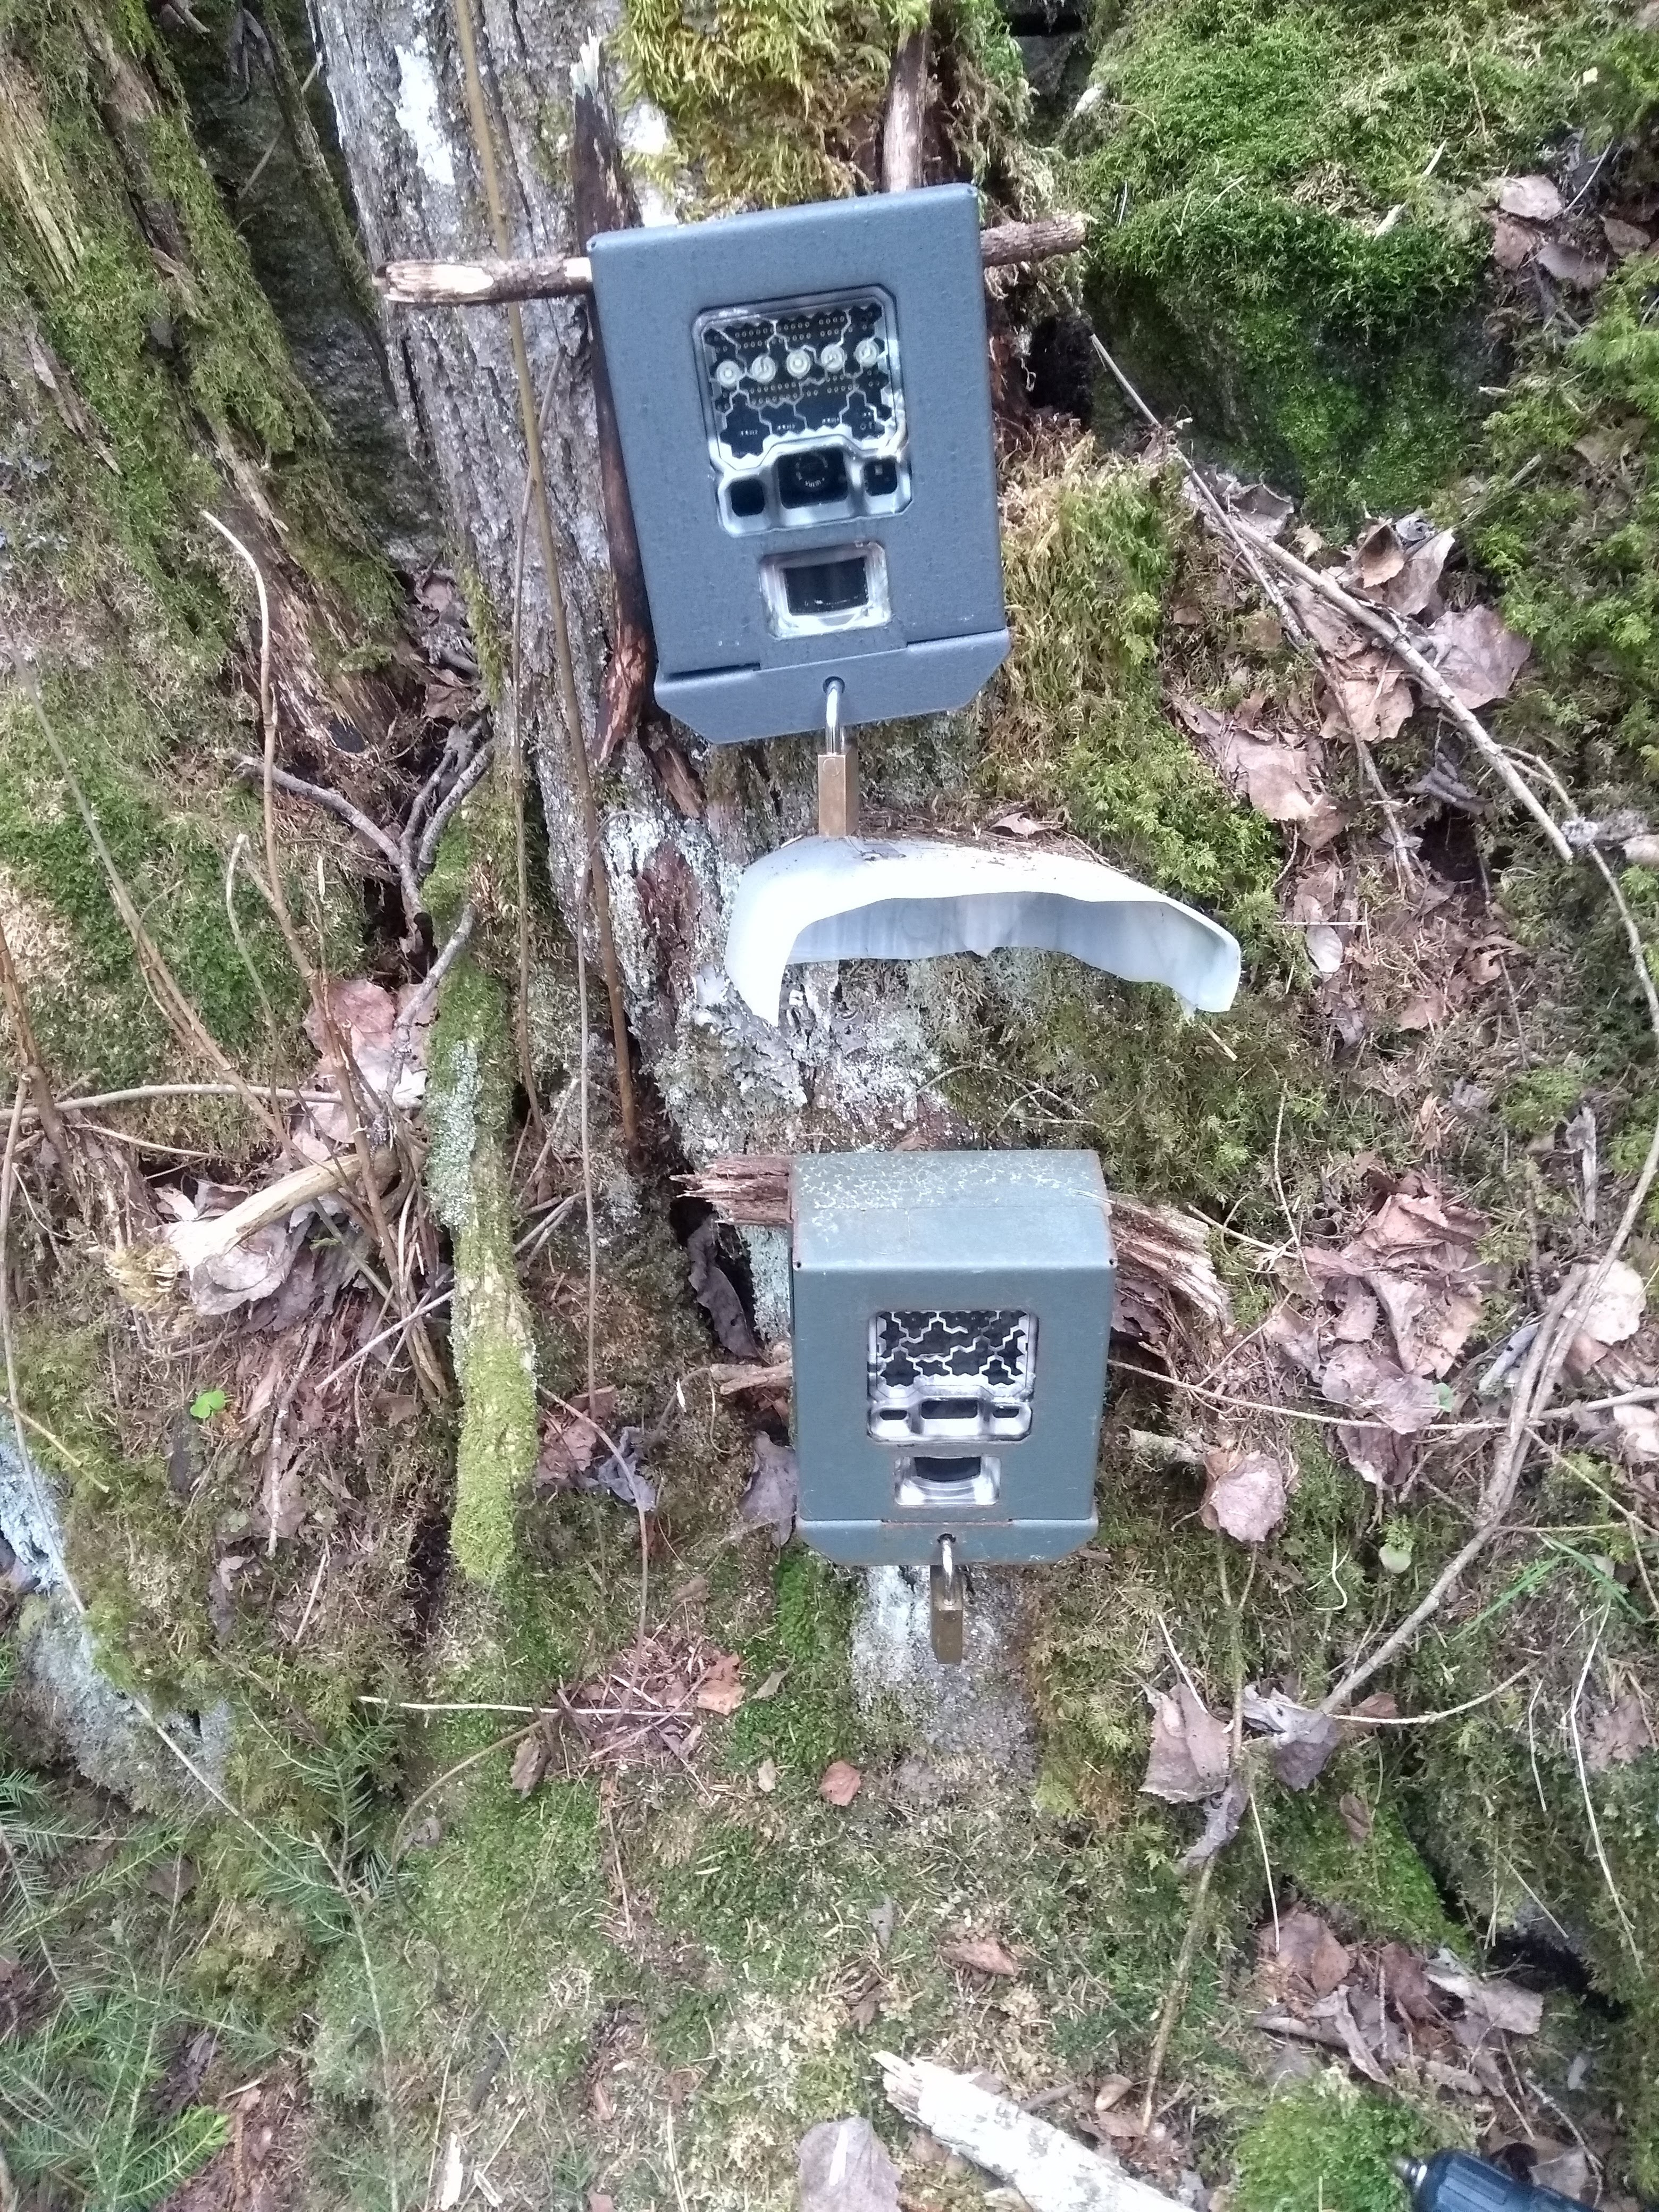
\includegraphics[width=.8\linewidth]{./img/cam_install_example/IMG_20190515_170952923.jpg}
		  \caption{Reconyx infrared,\\ installed with a snow cap}
		  	\label{fig:cam_ex_b}
	\end{subfigure}
		\begin{subfigure}{.5\textwidth}
		  \centering
		  	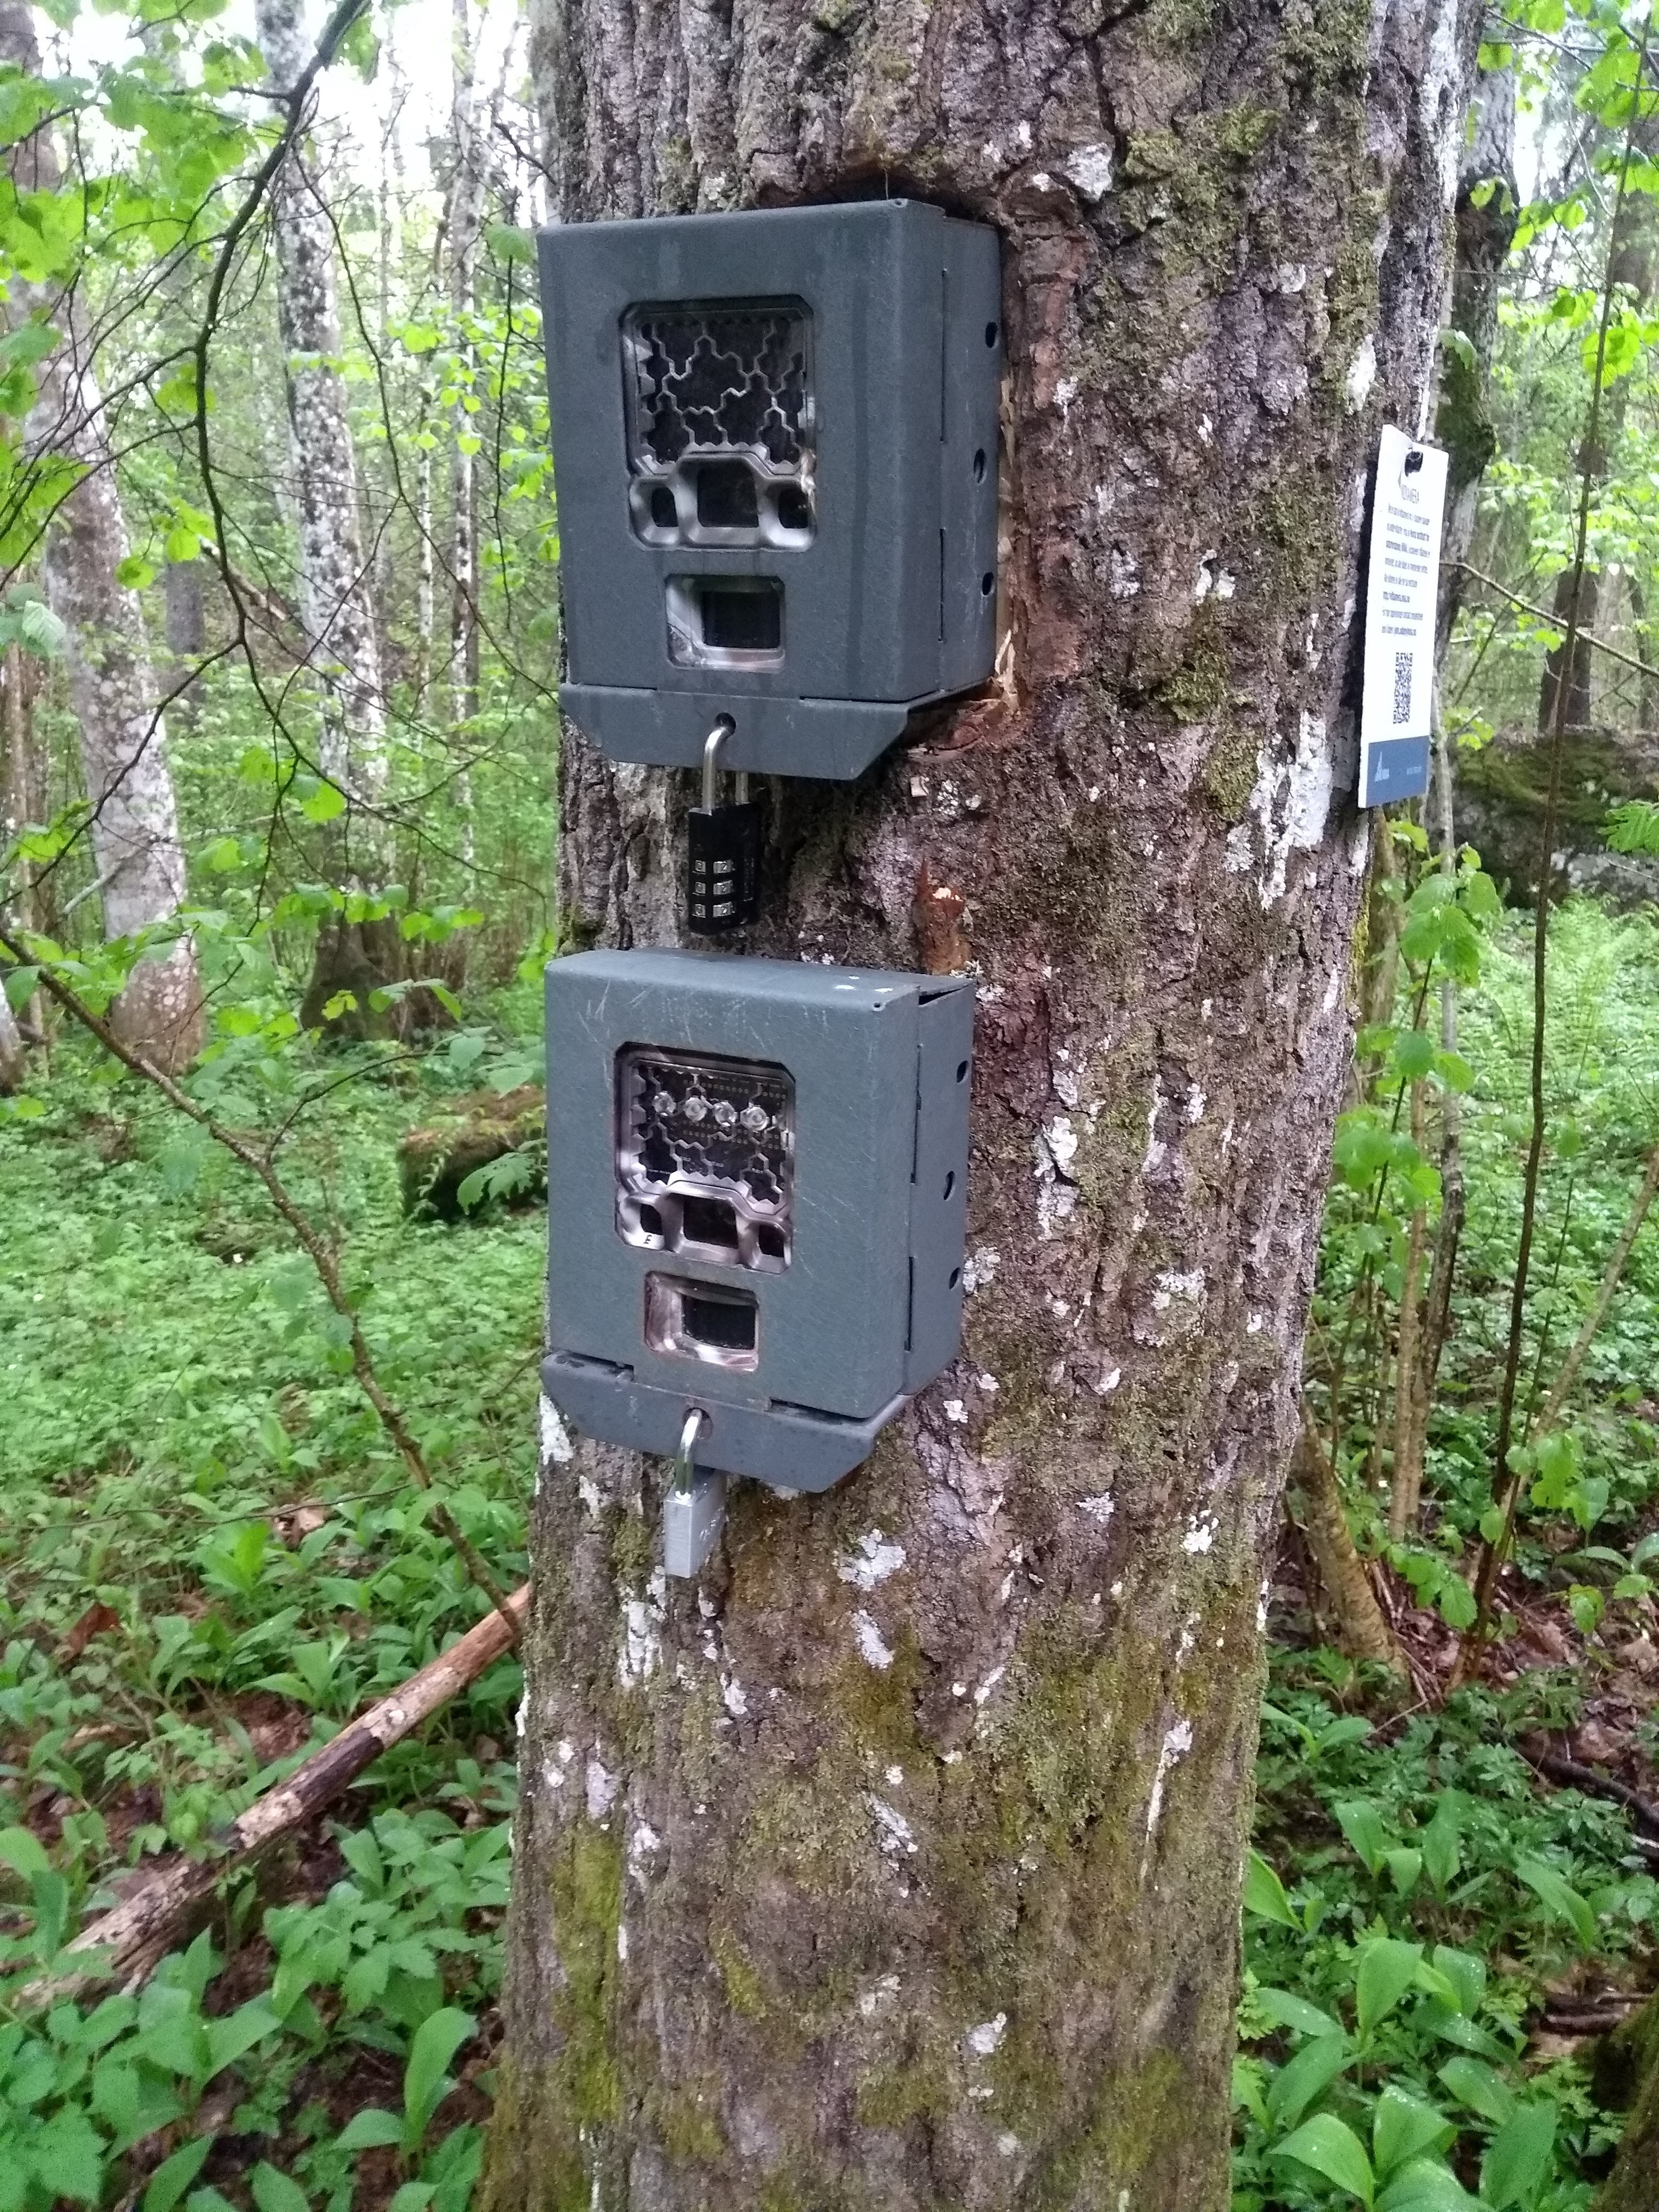
\includegraphics[width=.8\linewidth]{./img/cam_install_example/IMG_20190521_181329313.jpg}
		  \caption{Reconyx infrared above,\\ installed 160 cm above ground level}
		  	\label{fig:cam_ex_c}
	\end{subfigure}
		\begin{subfigure}{.5\textwidth}
		  \centering
		  	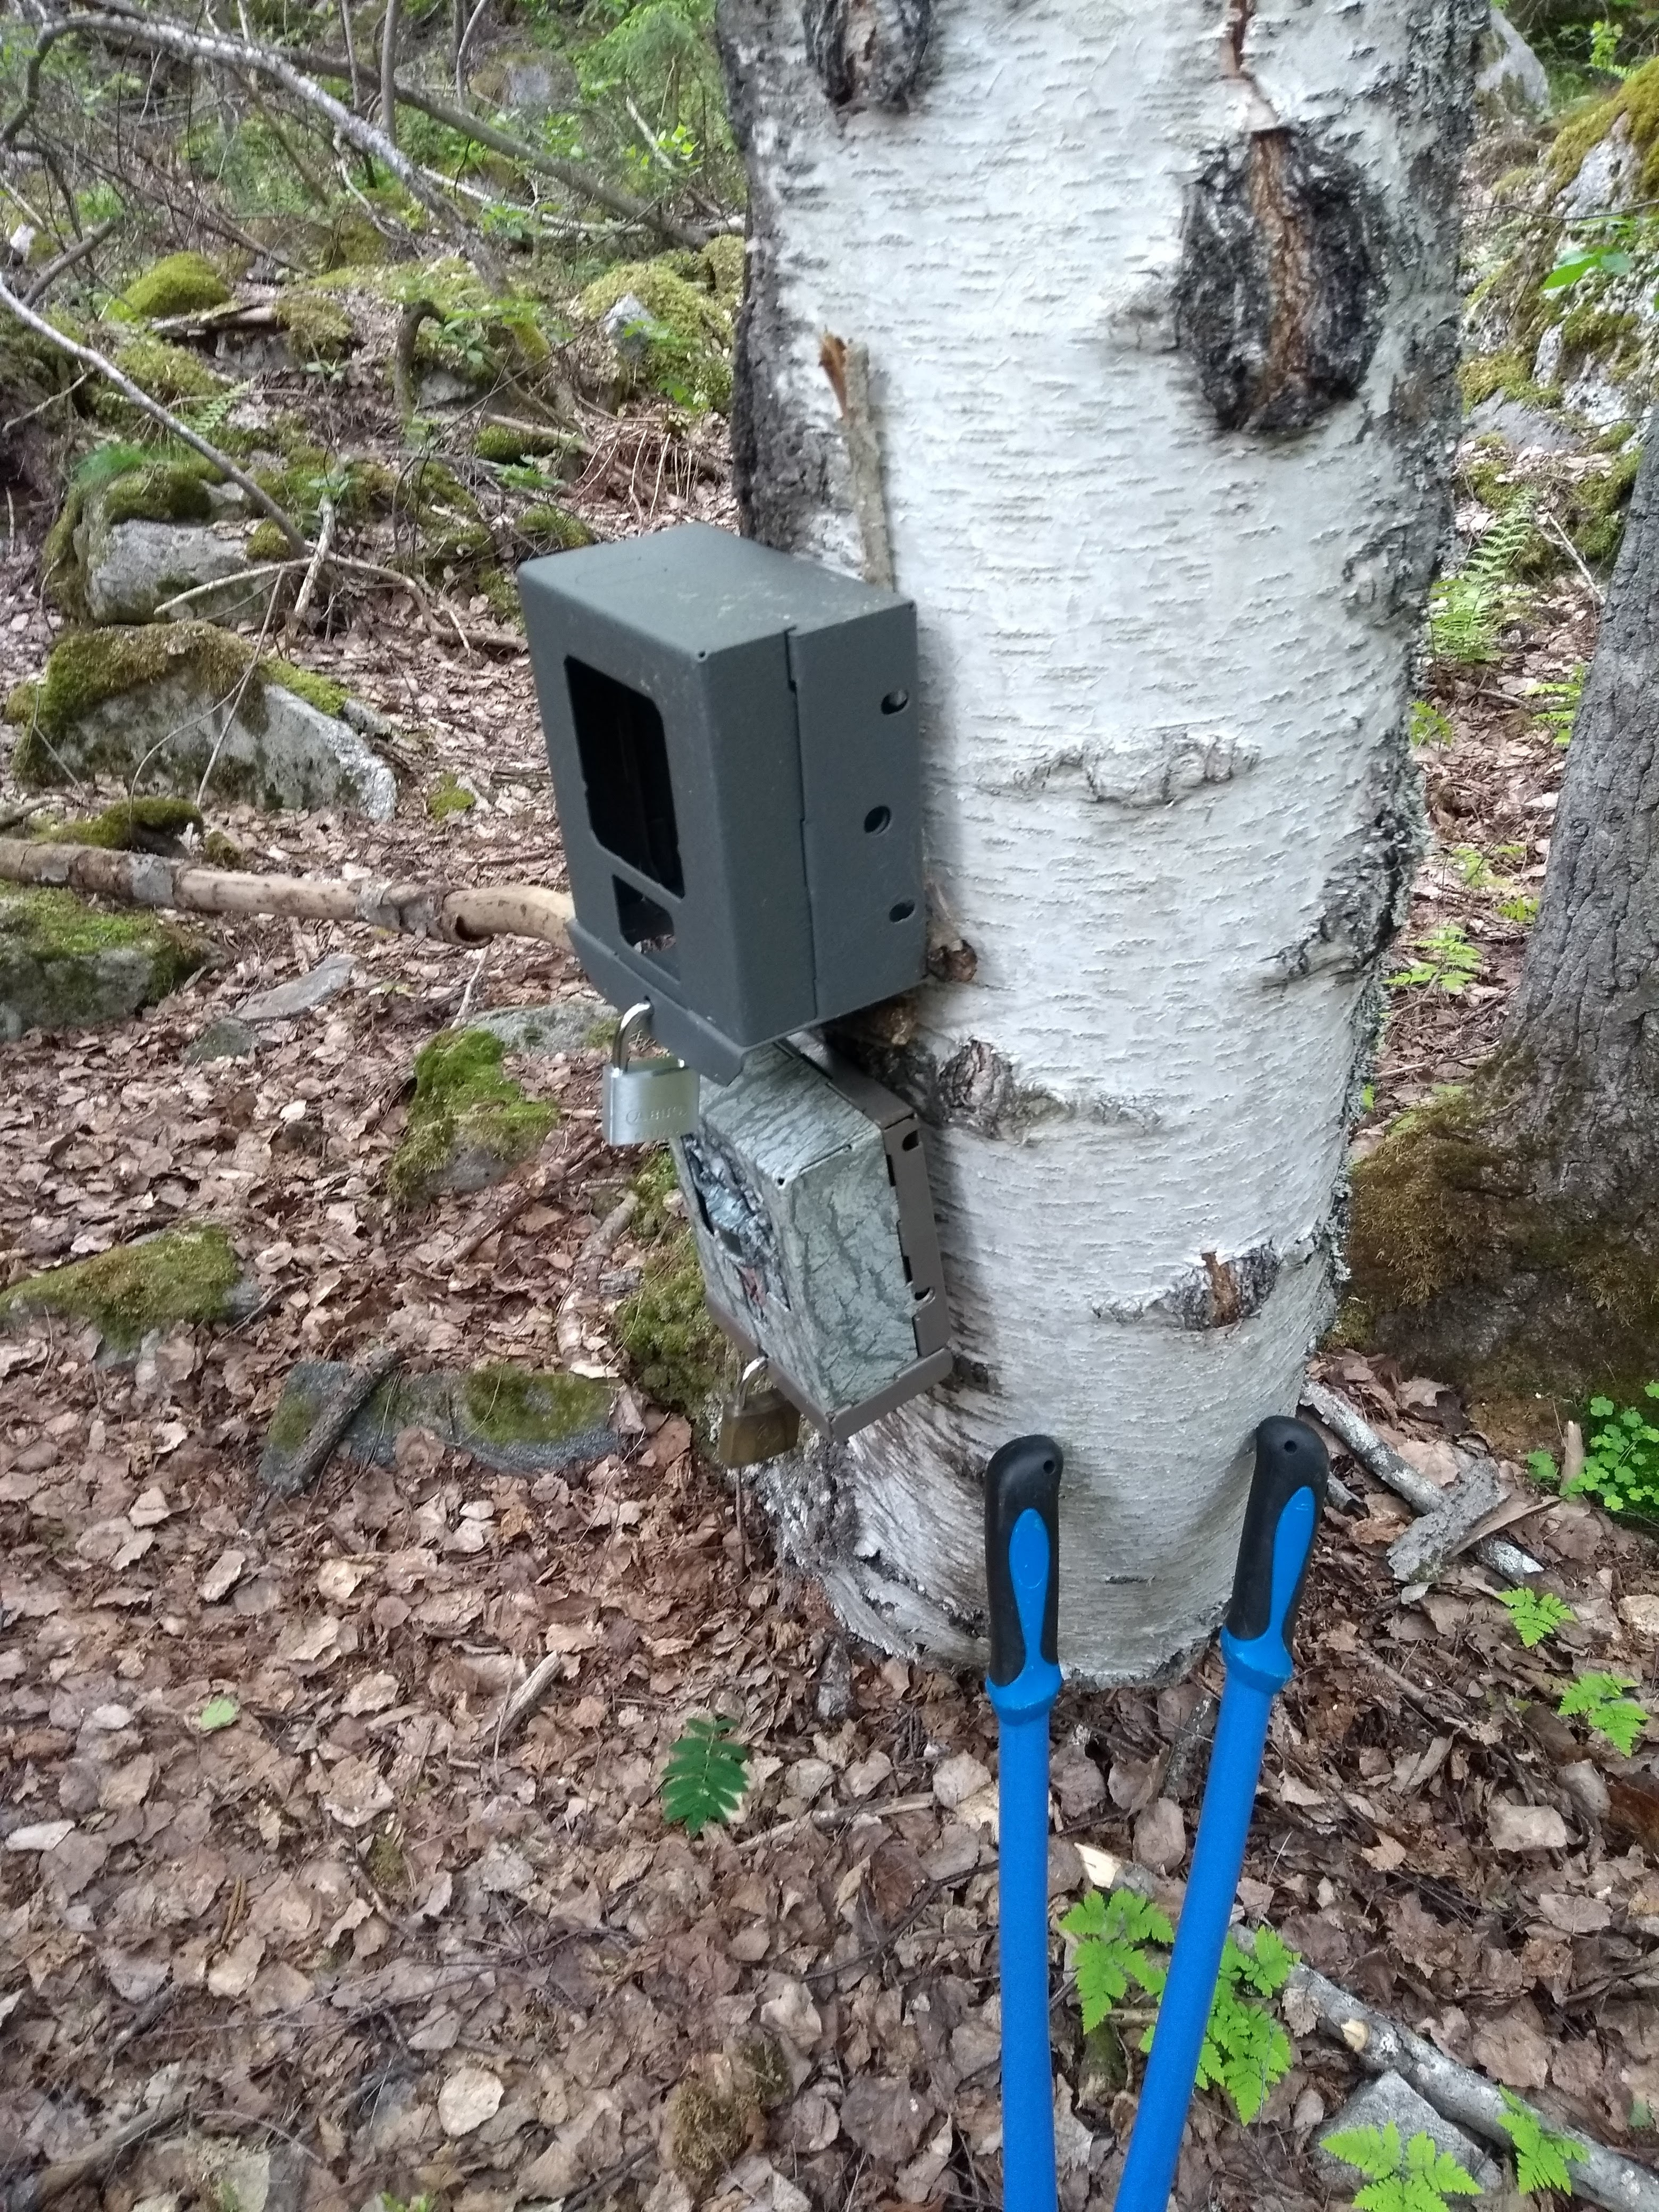
\includegraphics[width=.8\linewidth]{./img/cam_install_example/IMG_20190529_181049340.jpg}
		  \caption{Browning infrared,\\ white LED flash has just been removed}
		  	\label{fig:cam_ex_d}
	\end{subfigure}
		\caption{The preinstalled cameras varied in the way they were set up. Lower cameras with infrared, upper cameras with white LED (except in example c)}
	\label{fig:cam_ex_main}
\end{figure}

%We quantified the degree of consistency in implementing and reporting features of CT protocols and study design that might affect detectability and sampling error (e.g. camera type and settings, spatial and temporal sampling effort, use of attractants; Table S1). These details are fundamental to interpreting results of CT studies and assessing their reliability, repeatability and suitability for broader comparison or synthesis (Meek et al. 2014a)

%TODO Details of camera trap orientation, use of lures, and performance settings are also critical elements of camera trapping methodology. The height in relation to the target, the direction the camera is facing in relation to expected animal travel and path of the sun as well as horizontal and vertical alignment may all influence the results of camera trap studies. Providing clear descriptions of exactly how cameras were placed is fundamental to understanding and interpreting the results of research. (Meek etal 2014)





\section{Data Collection} %TODO  Trenger kilde på AI! 
%The fieldwork was conducted between September 15 and December 20, 2017. In this study, camera traps from the Norwegian Institute for Nature Research (NINA) were used. NINA uses camera traps to monitor the Eurasian lynx in southeastern Norway as part of the SCANDLYNX project (Odden, 2015). SCANDLYNX is a Scandinavian research project on the Eurasian lynx (Odden, 2015; SCANDLYNX, 2017). Camera traps were placed specifically with the goal to photo-capture lynx, and were therefore placed in steep terrain, on ledges or facing the cliff bases, often close to wildlife trails. The cameras were pointing perpendicular to the wildlife trail at locations where a wildlife trail was present. Each camera was mounted on a tree between 0.2 and 1 m above ground

Five different models of RECONYX™ (address: 3828 Creekside Ln, Ste 2, Holmen, WI 54636, USA, www.reconyx.com) cameras were used, 
and one model of BROWNING™ (address: One Browning Place, Morgan, UT 84050, USA, www.browningtrailcameras.com), details in table \ref{tab:cam_mod}.

Reconyx-cameras have been reported of having an average trigger speed of 0.2 seconds, whereas the Browning model was reported an average of 0.7 seconds (Trigger speed shootout, \cite{Trailcampro2014}).


\begin{table}
\caption{\label{tab:cam_mod} Camera models}
\centering

\begin{tabular}{llrrrr}
\hline
Producent  & Model name & Flash type & Trigger speed & photos/trigger & N \\
\cline{1-2}
\multirow{5}{2cm}{Reconyx HyperFire Series} &
	  HC500 Semi-Covert IR					& IR	& 0.2s & 3 & ? \\
	& HC600 High-Output Covert IR			& Black	& 0.2s & 3 & ? \\
    & PC800 Profoessional Semi-Covert IR 	& IR	& 0.2s & 3 & ? \\
    & PC900 Professional Covert IR 		& Black	& 0.2s & 3 & ? \\
    & PC850 Professional White Flash LED	& White	& 0.2s & 8 & 20 \\
\cline{1-2}
Browning  & Spec Ops: Extreme 				& IR	& 0.7s & ~ 24  \\
\hline
\end{tabular}

\end{table}



% [Detection shootout 2017](https://cdn.shopify.com/s/files/1/1065/8354/files/2017_Detection_Shootout_8de2600d-eb3a-42a8-9420-728aae5056e5.pdf?12422955367088316008)



Cameras were operating 24 hours per day. The RECONYX™ cameras were set to take one time lapse photo per day in order to verify that the cameras had been operational.
They were set to take 3 pictures per series, as fast as possible using \emph{rapidfire}, and retrigger immediately using \emph{no delay}.

The BROWNING™ cameras were also set to rapidfire, but to 8 photos per trigger, which unfortunately made the memory cards more vulnerable to filling up before being collected. This happened in some areas with sheep and/or cattle, and sometimes due to triggering by vegetation.

Therefore, the BROWNING™ cameras tended to have more gaps of inoperable days.
As seen in figure \ref{fig:map}, %TODO insert map with loc, white point inside flash-cameras.
there was a correlation between latitude and camera type.
In addition, there were a correlation between camera type and which trail type the cameras were put up in. BROWNING™ cameras were more frequently set up in trail types easily accessible by man, which in turn lead to more pictures of humans and vehicles on the browning cameras. %TODO insert plot of camera type on habitat and camera type on "human presence"


These differences should all be kept in mind when interpreting the models. 

% difference between the two camera types*** 
% Assumptions: chance of detection & sp validation BROWNING > RECONYX, operational days BROWNING < RECONYX



Whenever I noticed vegetation blocking the view of the camera, or excessively triggering it, I removed the vegetation.

\begin{figure}
	\label{fig:map}
\end{figure}




\section{Data processing} %TODO
All SD cards were delivered to NINA for data collection. Firstly, a facial recognition algorithm (FRA)  is used to sort all the pictures. %artificial intelligence software (AI)
Afterwards, a human sorter checks the softwares' output, confirming all the correct decisions (i.e. species detections) and correcting all the wrong ones.
The goal is to fully automate this process, which is a request from The Norwegian Data Protection Authority (DPA) in relation to usage of cameras in densely crowded areas (e.g. parks).
As per the four eyes principle, the detection rate of photographed species has gone up as a result of the FRA (pers.comm. John Odden). 

%Nei, vi har ikke publisert artikkel på gjenkjenningsalgoritmen. Du har jo vært med på prosessen sjøl, så jeg veit ikke om du egentlig trenger referanse her, men du kan sette inn John O som pers med og merke det, så kan han eller jeg endre det slik vi mener det bør være når vi leser gjennom oppgava di..


The output I got as a result, was a data frame containing a time stamp for every shutter activity, %kvar gong eit bilde blei tatt
including all meta data from the camera, coupled with predicted species (FRA output, with a confidence number), verified species (by human sorters), number of animals and distance from camera. The time stamps from the white flash cameras were used to verify whether an animal was in fact flashed or not, which I then used as my main predictor in the modelling. 
%Describing in brief how coding is undertaken is useful for readers to understand the methods used in relation to the results.(Meek etal 2014)


I defined one event as any 1 species passing with a buffer time of 5 min before or after %TODO  Må bestemme lengde på intervall, og formulere betre


The true number of active camera days are confounded by the lack of time lapse photos from the Browning cameras. To approach the true number of active days, I assumed all Browning cameras to be functional every day, unless the camera was inactive when I visited it. In that case, I considered the camera inactive since the day of its last photo.



%*************************************************************
%
%Hypothesis 1: Usage of white LED flash will stress one or more species in general, and therefore lower the detection rate of the stressed species. The effect will likely vary in extent between species.
%
%*************************************************************
%
%Hypothesis 2: The effect of the white LED will correlate with urbanisation-factors, as individuals that live closer to urban areas are habituated to Artificial Light At Night (ALAN), and thus will have a weaker response to the white LED
%
%


\section{Statistical analysis} %This is a reference to the session info appendix \ref{app:sessinfo}

To test for effects of the white LED flash I used the R programming language (\cite{RCoreTeam2020}), in the RStudio IDE (\cite{RStudioTeam2020a}), adopting large parts of the tidyverse framework along the way (\cite{tidyverse}). Session info in appendix \ref{app:sessinfo}. %Atle: Why sessioninfo?
%TODO easystats også, etterkvart.


	\subsection*{GLMM}
To test $H_{1}$ I looked for differences in detection rate per day, using Generalised Linear Mixed Models (GLMM) with the glmer function from the R package lme4 (\cite{lme4}).

Generalised Linear Model, because my dependent variable was count data, which I assume follows a Poisson distribution ($ X \sim Pois(\lambda) $).
Mixed effects to include location ID and week of the year as random effects, accounting for differences between camera sites, and seasonal changes during the year of study.

Consequently, I fitted a poisson mixed model (estimated using Maximum Likelihood and Nelder-Mead optimizer) on a subset of each species, to predict number of observations, with time since deployment in days interacting with flash type (formula: n.obs ~ time.deploy * flash).

Standardized parameters were obtained by fitting the models on standardized versions of the data subset. 95\% Confidence Intervals (CIs) and p-values were computed using the Wald approximation. % for results: Predicted counts visualised in \vref{fig:glmm_sp}, model parameters visualised in \vref{fig:para_sp}.

The flash type-variable corresponds to white LED present/absent or control group.
For the cameras that was equipped with an additional white LED camera, time since deployment starts from the day I visited the camera, and set up/ took down the white LED.
The control group’s “day 0” of time since deployment were set by me when doing the analysis, at points reflecting my weeks of field work, in order to obtain periods of similar lengths to that of the white LED-locations. See 
Further, I also trimmed the period lengths down to a reduced length, based on the median length of the IR and white LED periods. Thus, any period exceeding the shortest median length, was trimmed down, as visualized in \ref{fig:median_period}. 



\begin{figure}
\caption{\label{fig:median_period} Period lengths}
	\centering
	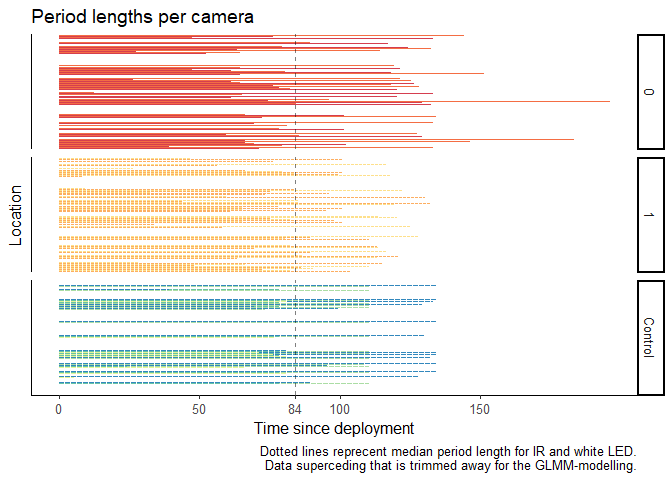
\includegraphics[scale=.8]{../R/glmm_sp_files/figure-gfm/period-length-wControl-1.png}
\end{figure}


\begin{figure}
	\begin{subfigure}{1\textwidth}
		\centering
		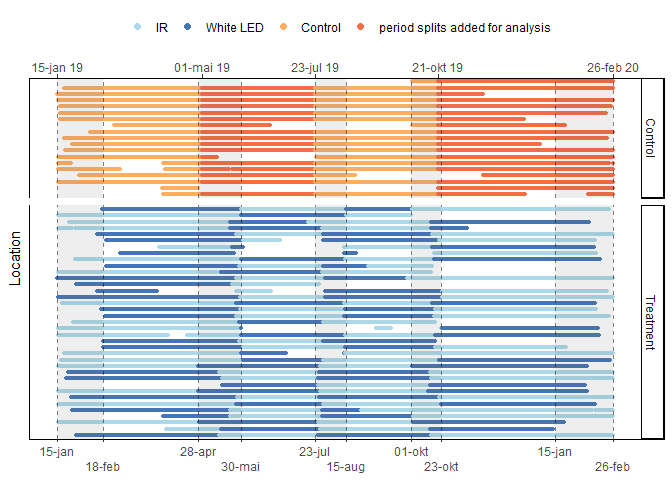
\includegraphics[scale=.8]{../R/FLM_notebook_files/figure-gfm/effort-facet-1.png}
			\caption{\label{fig:timeseries_flash} Cameras with white LED periods}	
	\end{subfigure}	
	\begin{subfigure}{1\textwidth}
		\centering
		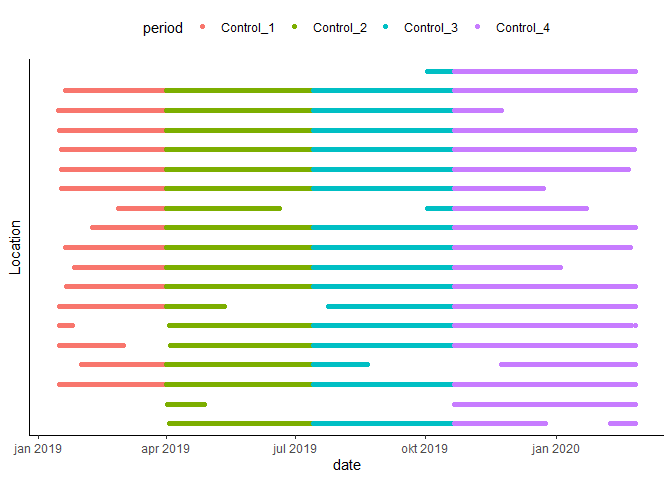
\includegraphics[scale=.8]{../R/FLM_notebook_files/figure-gfm/effort-facet-2.png}
			\caption{\label{fig:timeseries_control} Control cameras'\\ period breaks were set during the analysis.}	
	\end{subfigure}	
\caption[Active camera days]
{Colours indicate the different periods for each camera. Control camera periods were defined in similar lengths to that of the cameras that had periods with an additional white LED CT. Thus, "day 0" of Control-cameras are often set at dates far from an actual visitation day. \label{fig:timeseries_figure}}
\end{figure}



%### report output
I fitted a poisson mixed model (estimated using Maximum Likelihood and Nelder-Mead optimizer) to predict number of observations with time since deployment and flash type (formula: n.obs ~ time.deploy * flash).
The model included location ID and week as random effects (formula: list(~1 | loc, ~1 | week)).


%Standardized parameters were obtained by fitting the model on a standardized version of the dataset. 95\% Confidence Intervals (CIs) and p-values were computed using the Wald approximation. Predicted counts visualised in \vref{fig:glmm_sp}, model parameters visualised in \vref{fig:para_sp}.




%\begin{align*}
%   n.obs \sim               && \text{Dependant variable}\\
%   time  \times flash       && \text{predicted by fixed effects}\\
%   + (1|loc) + (1|week)     && \text{controlling for random effects}\\
%\end{align*} 


\subsection{Equivalence test}
% Multiple testing i arkiv/method-ark
I used the standard significance level of $\alpha = .05$, and performed an equivalence test on my model outputs, using the function equivalence-test from the R package parameters ().%\cite{package-parameters}). %TODO

In an equivalence test, model parameters are tested against a Region of Practical Equivalence (ROPE) as opposed to merely one single mean value, thus accounting for the \emph{effect size} of each parameter.
If the parameters estimate and CI falls outside the ROPE, their null hypothesis is rejected. However, if the CI is inside the ROPE, H0 is accepted, no matter if a standard Null Hypothesis Significance Test (NHST) would have deemed it significant.

Inside the function equivalence-test I used the Two One-Sided Tests (TOST) rule, where the confidence interval (CI) is set to $1 - 2\times \alpha$. In my case that gave a narrow CI of .90,

For models from count data, the residual variance is often used to define the ROPE range. However, the description of the rope-range function from the package bayestestR () states this threshold as "rather experimental" and that the range is probably often similar to the default [-0.1, 0.1] of a standardized parameter.
Hence, I used the default ROPE range which corresponds to a negligible effect size according to Cohen, 1988.

%In the TOST procedure, the null hypothesis is the presence of a true effect of DL or DU, and the alternative hypothesis is an effect that falls within the equivalence bounds or the absence of an effect that is worthwhile to examine. \cite{Lakens2017}








	\subsection*{Cox Proportional Hazards}
%What I am in truth testing is each camera's chance of contracting a roe deer disease, or fox disease, and how that chance changes when "treated" with a white LED flash.


However, the way I set up the GLMMs, it only takes into account whether a flash was present or not. It can't tell if the flash actually went off, or how many times it did.


Therefore I set up a new column in my dataset called flashed, that told if the flash went off in synchrony with the IR camera.
I then used the flashed-column to set up a time to event-analysis.

Also called Survival analysis, time to event-analyses compares groups' risk of experiencing an event, and was first developed for use in medicinal studies (e.g. cancer risk studies).

The difference between the groups is called the hazard \emph{ratio}, and is \emph{assumed to be proportional} over time. That is, if after 2 days, the hazard of detecting a fox (i.e. experiencing an event) for the IR-group is twice as large compared to the white LED-group, it should remain twice as large after 25 days as well. Or in other words, the IR-group should detect twice as many foxes as the white LED-group in general.


The Cox proportional hazards regression model (CPH model) (Cox, 1972), is a popular development of the time to event-analysis because it allows for more than one predictor. I used the R package Survival (\cite{survival-package}) and the function coxme from the R package coxme \cite{coxme-package} to perform a CPH with mixed effects (fixed and random effects). 

Again, location ID and week of the year were used as random effects to account for differences between the camera sites and seasonal changes during the study period.


As fixed effect I used the flashed-column.
If a species was flashed, it went into the "flashed"-group, and time to next detection was recorded. 
If the species didn't reappear it was "censored" from the model.


In survival-analyses the time-variable is part of the outcome of the model. Event (i.e. detection) and time is joined as a Surv-object by the Surv function from the Survival package. 


Both these models told me something about the fallacy of $H_0$, whether I could reject it, or fail to reject it.
If the null hypothesis was rejected for a species, I considered $H_1$ to be true. Then I went on to test $H_2$





	\subsection*{P-tests and assumptions}

For both the GLMM and the CPH mixed effect model, I used the Wald test as significance test, with xyz distribution over df degrees of freedom. osvosv. 


%Attention devoted to model assumptions! Viktig i Burton 2015
The R package performance (cite) was used to check assumptions for GLMM, and ggeffects (cite) was used to visualize the results. 

R package Survminer was used to visualize the results of the time to event analyses.
The Schoenfeld test was used to check for the CPH's assumption of proportional hazards. 



%\subsection{AIC old}

%If you are using AIC model selection in your research, you can state this in your methods section. Report that you used AIC model selection, briefly explain the best-fit model you found, and state the AIC weight of the model.

%For each species, I used the Akaike Information Criterion (AIC) to select the best models excluding the flashed-predictor.
%Then, I added the flashed-predictor to each species top model, to see whether this effect could account for any remaining variation.
%
%
%Example: 
%
%We used AIC model selection to distinguish among a set of possible models describing the relationship between age, sex, sweetened beverage consumption, and body mass index.
%The best-fit model, carrying 97\% of the cumulative model weight, included every parameter with no interaction effects.

%After finding the best-fit model you can go ahead and run the model and evaluate the results. The output of your model evaluation can be reported in the results section of your paper.


